\documentclass[conference]{IEEEtran}
\usepackage{cite,amsmath,graphicx,booktabs,array,url}
\begin{document}

\title{Forest Fire and Smoke Detection with a Vision-Transformer Backbone: \\ A ViTDet-Style Faster R-CNN Evaluated on the D-Fire Dataset}

\author{\IEEEauthorblockN{[Author name]}
\IEEEauthorblockA{[Department, Institution]\\
[City, Country]\\
[Email]}}

\maketitle

\begin{abstract}
Early detection of forest fires depends on finding both fire and the smoke that often precedes it in ordinary camera images. This paper presents a detector that uses a plain Vision Transformer (ViT) backbone with a simple feature pyramid and a Faster R-CNN head, following the ViTDet design, and evaluates it on the D-Fire dataset (14{,}122 training, 3{,}099 validation and 4{,}306 test images, two classes: smoke and fire). Architecture and training recipe were chosen with short comparison runs on a subset, and inference thresholds were tuned on validation data only. On the held-out test set the final model reaches 78.07\% mAP@0.50 and 41.22\% mAP@0.50:0.95, with 85.33\% AP@0.50 for smoke and 70.81\% for fire. The result falls 11.93 points short of the 90\% mAP@0.50 target set at the start of the project. An error analysis shows that the shortfall is concentrated in fire: small fire regions have 52.5\% recall and 478 fire detections were rejected for poor localisation, while false alarms on images with no fire or smoke are rare (1.3\%). All results come from a single training run with one random seed.
\end{abstract}

\begin{IEEEkeywords}
forest fire detection, smoke detection, object detection, Vision Transformer, Faster R-CNN, D-Fire
\end{IEEEkeywords}

\section{Introduction}
Wildfires cause large losses, and the time between ignition and detection strongly affects how far a fire spreads. Cameras on towers and drones provide a cheap source of imagery, but reliable automatic detection is difficult: smoke is diffuse and varies in shape and colour, early fire regions are tiny, and many scenes contain sun glare, clouds, fog or lights that resemble fire and smoke.

Convolutional detectors are the usual choice for this task. Plain Vision Transformers~\cite{dosovitskiy2021vit} offer a different backbone whose pretrained weights are widely available, and ViTDet~\cite{li2022vitdet} showed that a plain ViT can serve as a detection backbone when a simple feature pyramid is built from its single-scale output. Fire detection is a natural test of this idea, because it needs both large-context reasoning (smoke) and fine detail (small flames).

This work makes the following contributions:
\begin{itemize}
\item A ViTDet-style Faster R-CNN~\cite{ren2015faster} for smoke and fire detection, with anchors selected from the box statistics of the training data.
\item A two-stage selection procedure that compares backbone size, input resolution, pyramid depth, layer freezing and two training recipes on a subset before the final training.
\item A test-set evaluation with class-wise precision, recall, F1 and AP, and an error breakdown by error type and object size.
\item An honest account of where the model falls short of a 90\% mAP@0.50 target.
\end{itemize}

\section{Related Work}
\textbf{Object detection.} Faster R-CNN~\cite{ren2015faster} combines a region proposal network with a region-based classifier and box regressor and remains a strong two-stage baseline. Detection quality is commonly reported with the COCO average-precision protocol~\cite{lin2014coco}.

\textbf{Transformers for detection.} ViT~\cite{dosovitskiy2021vit} splits an image into patches and processes them with global self-attention. ViTDet~\cite{li2022vitdet} adapts a plain ViT to detection by building a multi-scale pyramid from the final stride-16 feature map with simple (de)convolutions, and this paper follows that design.

\textbf{Fire and smoke detection.} The D-Fire dataset~\cite{venancio2022dfire} provides images with bounding boxes for smoke and fire, including many images with neither. It is the dataset used here.

\section{Dataset}
D-Fire in YOLO format is used with two classes, smoke and fire. Table~\ref{tab:data} gives the split sizes. About 45\% of the images in every split have empty label files. These show scenes without fire or smoke and are kept as negative examples. The three splits share no file names.

\begin{table}[t]
\centering
\caption{Dataset splits after label cleaning.}
\label{tab:data}
\begin{tabular}{lrrrrr}
\toprule
Split & Images & Empty & Boxes & Smoke & Fire \\
\midrule
Train & 14{,}122 & 6{,}458 & 17{,}418 & 7{,}788 & 9{,}630 \\
Val   & 3{,}099  & 1{,}375 & 3{,}930  & 1{,}754 & 2{,}176 \\
Test  & 4{,}306  & 2{,}005 & 5{,}189  & 2{,}311 & 2{,}878 \\
\bottomrule
\end{tabular}
\end{table}

Labels were converted from normalised centre format to pixel corners. Coordinates outside the image were clipped (284 boxes), boxes narrower than 2 pixels were removed (20 boxes), and exact duplicates and malformed lines were dropped. The most common training resolutions are $1280\times720$ (6{,}062 images) and $640\times360$ (2{,}724 images). Objects are divided into size buckets by box-to-image area ratio: small below 0.52\%, medium from 0.52\% to 6.09\%, and large above 6.09\%.

\section{Method}
\subsection{Architecture}
The detector has three parts. The backbone is a plain ViT with patch size 16, pretrained on ImageNet-21k and fine-tuned on ImageNet-1k (\texttt{augreg} weights from the \texttt{timm} library), which is then fine-tuned end to end on D-Fire. A simple feature pyramid built from the single stride-16 map produces levels at strides 4, 8, 16 and 32, plus one extra pooled level for the region proposal network. Global self-attention is used in every block. The head is the Faster R-CNN implementation in \texttt{torchvision} with RoIAlign.

Anchor sizes are $k\times$ stride at each pyramid level. Candidate settings were scored by the mean IoU between each training box and its best-matching centred anchor, under a budget of six anchors per location. The selected setting uses $k\in\{4,6\}$ with aspect ratios $\{0.5,1,2\}$, giving a mean best IoU of 0.741 and 92.2\% of training boxes with an anchor at IoU~$\ge0.5$.

\subsection{Preprocessing and augmentation}
Images are letterboxed to a $640\times384$ canvas with aspect ratio preserved, so predicted boxes map back to the original image by a single division by the scale. Training augmentation consists of horizontal flips, random scale and translation, brightness and contrast changes, mild hue and saturation changes, blur and noise. Vertical flips and strong colour shifts are avoided because fire and smoke appearance depends on colour. Each epoch uses all images that contain objects and a freshly sampled fraction of the empty images.

\subsection{Optimisation}
Training uses AdamW~\cite{loshchilov2019adamw} with weight decay 0.05, which is not applied to normalisation layers, biases or position embeddings. Layer-wise learning-rate decay of 0.8 makes early ViT blocks change more slowly than the pyramid and heads. A linear warm-up of 300 iterations is followed by cosine decay, and gradients are clipped. The ViT and pyramid run in fp16 mixed precision, while the region proposal network, box head and losses run in fp32. Drop-path is 0.1. An exponential moving average of the weights (decay 0.999) is used for validation and saved as the final model. The batch size is 8.

\subsection{Model selection}
Selection used a 2{,}000-image training subset and a 500-image validation subset, with 3 epochs per candidate. Stage~A compared architecture, resolution and fine-tuning strategy. Stage~B compared two recipe changes on the Stage~A winner. Short runs give only a relative ranking, so they were used solely to choose the final configuration.

\subsection{Inference settings}
Two settings were tuned on validation data only, never on test data: the non-maximum-suppression IoU threshold, chosen by validation mAP@0.50, and the confidence threshold, chosen to maximise the mean per-class F1 at IoU 0.5. The selected values are 0.5 and 0.82.

\section{Experimental Setup}
All experiments ran on a single AMD Radeon RX 9070 GRE GPU using a ROCm build of PyTorch 2.9.1, with \texttt{torchvision} 0.24.1, \texttt{timm} 1.0.29 and \texttt{albumentations} 2.0.8. The random seed was 42 and each configuration was run once. Model selection took about 78 minutes and the final training took 200 minutes.

\textbf{Metrics.} AP@0.50, mAP@0.50 and mAP@0.50:0.95 follow the COCO protocol~\cite{lin2014coco} with 101-point interpolation. Precision, recall and F1 are computed by matching detections to ground truth greedily by confidence at IoU 0.5, with each ground-truth box matched once and the class required to agree, at the single confidence threshold above. Overall precision, recall and F1 are macro-averages over the two classes. Accuracy is not reported because it is not a detection metric.

\section{Results}
\subsection{Model selection}
Table~\ref{tab:stagea} shows Stage~A. The ViT-B backbone at $640\times384$ was best. The larger $832\times480$ input was slower and scored lower than the base setting in this short run, and freezing early blocks or removing the stride-4 level scored lower. In Stage~B (Table~\ref{tab:stageb}), a learning rate of $2\times10^{-4}$ scored highest, although the three recipes lie within 1.3 points of each other, so this is a mild preference rather than a decisive one.

\begin{table}[t]
\centering
\caption{Stage A: architecture selection (3 epochs, 2{,}000 training images, validation subset of 500 images).}
\label{tab:stagea}
\begin{tabular}{lrrr}
\toprule
Configuration & mAP@50 & mAP@50:95 & Min \\
\midrule
ViT-B, $640\times384$ & \textbf{49.61} & \textbf{20.32} & 11.7 \\
ViT-S, $640\times384$ & 45.07 & 16.59 & 10.9 \\
ViT-S, $832\times480$ & 43.05 & 15.76 & 28.7 \\
ViT-S, no stride-4 level & 38.82 & 14.64 & 5.3 \\
ViT-S, first 6 blocks frozen & 38.62 & 13.93 & 5.4 \\
\bottomrule
\end{tabular}
\end{table}

\begin{table}[t]
\centering
\caption{Stage B: training recipe on ViT-B.}
\label{tab:stageb}
\begin{tabular}{lrrr}
\toprule
Recipe & mAP@50 & mAP@50:95 & Min \\
\midrule
Learning rate $2\times10^{-4}$ & \textbf{50.68} & \textbf{20.76} & 7.0 \\
Baseline (lr $1\times10^{-4}$) & 49.61 & 20.32 & 11.7 \\
All negatives every epoch & 49.41 & 20.50 & 9.0 \\
\bottomrule
\end{tabular}
\end{table}

\subsection{Final training}
The final model is ViT-B at $640\times384$ with learning rate $2\times10^{-4}$, trained on the full training set for 12 epochs with early stopping after 4 epochs without improvement (not triggered). Validation mAP@0.50 rose from 56.57 after epoch 1 to 79.03 at epoch 8 and then stayed between 78.79 and 79.15 (Fig.~\ref{fig:curves}), while the training loss kept falling from 0.251 to 0.234 over epochs 9 to 12. The best checkpoint, from epoch 10, has validation mAP@0.50 of 79.15\% and mAP@0.50:0.95 of 41.93\%.

\begin{figure}[t]
\centering
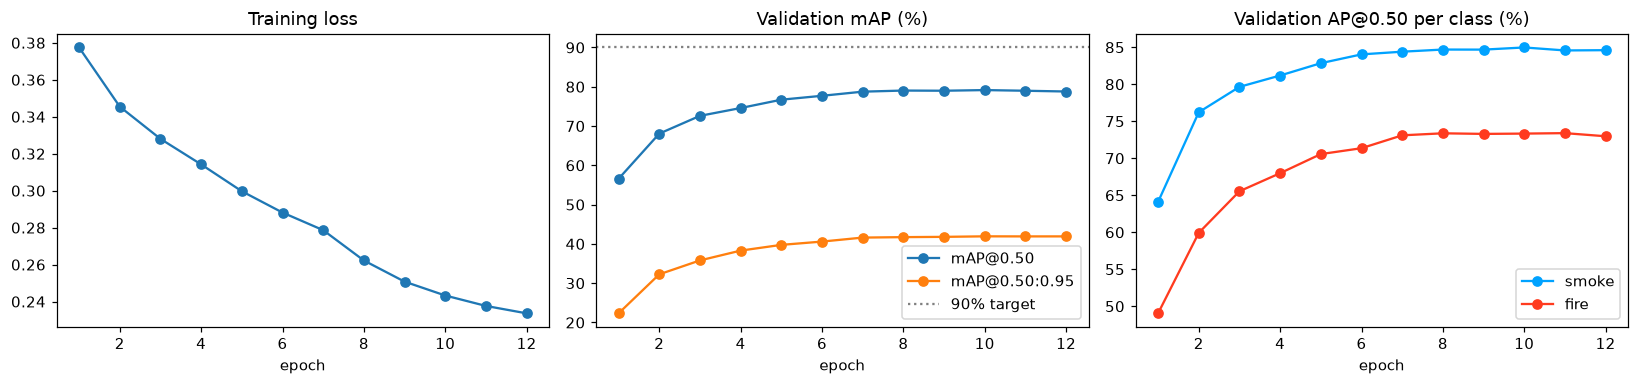
\includegraphics[width=\columnwidth]{training_curves.png}
\caption{Training loss, validation mAP and per-class validation AP@0.50 over the 12 epochs of final training.}
\label{fig:curves}
\end{figure}

\subsection{Test results}
Table~\ref{tab:test} reports test-set results. Overall mAP@0.50 is 78.07\% and mAP@0.50:0.95 is 41.22\%, close to the validation values, so the tuned thresholds and selected checkpoint do not appear to be overfitted to the validation set. Smoke is detected more reliably than fire on every metric. Fig.~\ref{fig:pr} shows the precision--recall curves and the F1 behaviour around the chosen confidence threshold.

\begin{table}[t]
\centering
\caption{Test-set results (4{,}306 images; confidence 0.82, NMS IoU 0.5, match IoU 0.5).}
\label{tab:test}
\begin{tabular}{lrrrrr}
\toprule
Class & P & R & F1 & AP@50 & AP@50:95 \\
\midrule
Smoke & 82.35 & 83.56 & 82.95 & 85.33 & 48.12 \\
Fire  & 73.04 & 65.43 & 69.02 & 70.81 & 34.32 \\
Overall & 77.69 & 74.49 & 75.99 & 78.07 & 41.22 \\
\bottomrule
\end{tabular}
\end{table}

\begin{figure}[t]
\centering
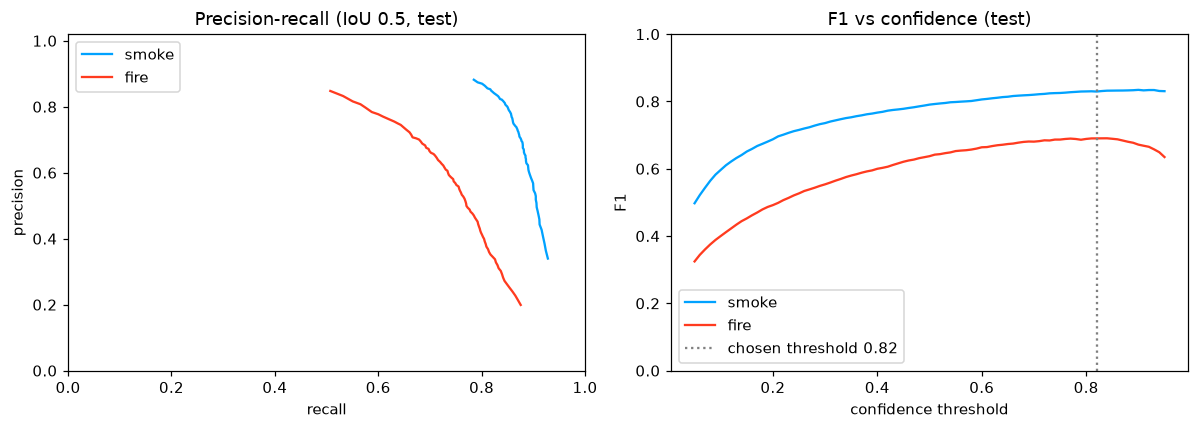
\includegraphics[width=\columnwidth]{test_pr_f1_curves.png}
\caption{Test precision--recall curves at IoU 0.5 and F1 versus confidence threshold; the dotted line marks the chosen threshold of 0.82.}
\label{fig:pr}
\end{figure}

\subsection{Error analysis}
Every test detection above the confidence threshold was matched to ground truth at IoU 0.5 and categorised (Table~\ref{tab:err}). Poorly localised boxes (right class, IoU between 0.1 and 0.5) are the largest source of false positives, especially for fire (478 boxes). Misses are also concentrated in fire, with 983 missed fire boxes against 375 for smoke. Confusion between the two classes is rare.

\begin{table}[t]
\centering
\caption{Test errors at the chosen confidence threshold.}
\label{tab:err}
\begin{tabular}{lrr}
\toprule
Error type & Fire & Smoke \\
\midrule
FP: poor localisation & 478 & 266 \\
FP: background & 192 & 127 \\
FP: duplicate & 20 & 6 \\
FP: wrong class & 5 & 15 \\
FN: missed & 983 & 375 \\
FN: class confusion & 12 & 5 \\
\bottomrule
\end{tabular}
\end{table}

Recall depends strongly on object size (Table~\ref{tab:size}). Fire recall is 52.5\% for small objects against 80.6\% for large ones, which is the clearest weakness of the model. Of the 2{,}005 empty test images, only 27 (1.3\%) produced at least one false alarm.

\begin{table}[t]
\centering
\caption{Test recall (\%) by object size.}
\label{tab:size}
\begin{tabular}{lrrr}
\toprule
Class & Small & Medium & Large \\
\midrule
Fire  & 52.5 & 77.5 & 80.6 \\
Smoke & 67.6 & 75.7 & 90.5 \\
\bottomrule
\end{tabular}
\end{table}

\section{Discussion and Limitations}
The model reaches 78.07\% mAP@0.50 and does not meet the 90\% target. Validation performance flattened after epoch 8 while the training loss continued to fall, so simply training longer with the same setup is unlikely to close the gap. The error analysis points to small and poorly localised fire as the main causes. Higher input resolution and a stronger pyramid are plausible remedies, but the one higher-resolution candidate tested ($832\times480$) scored lower in a short run, so this remains untested at full length.

Limitations should be kept in mind. All results come from one training run with one seed, so differences of a point or so, including the Stage~B recipe ranking, are within what run-to-run variation could produce. Selection used short runs on a subset, which may not rank configurations the way full training would. The study evaluates a single dataset and compares no other detectors, such as YOLO-family models, under the same protocol, so no claim is made that this approach is better or worse than convolutional alternatives. Inference speed and memory use were not measured, so suitability for embedded deployment is not established.

\section{Conclusion}
A ViTDet-style Faster R-CNN with a ViT-B backbone was trained and evaluated for smoke and fire detection on D-Fire. It achieved 78.07\% mAP@0.50 on the test set, with smoke (85.33\% AP@0.50) detected better than fire (70.81\%). The main weakness is small fire regions. Future work includes higher-resolution input, a comparison against convolutional detectors under the same protocol, repeated runs with different seeds, and measurement of inference speed.

\section*{Availability}
The complete code, the trained checkpoint and the logs of this run are available from the author on request. The dataset is publicly available as D-Fire.

\begin{thebibliography}{00}
\bibitem{dosovitskiy2021vit} A. Dosovitskiy \emph{et al.}, ``An image is worth 16x16 words: Transformers for image recognition at scale,'' in \emph{Proc. ICLR}, 2021.
\bibitem{li2022vitdet} Y. Li, H. Mao, R. Girshick, and K. He, ``Exploring plain vision transformer backbones for object detection,'' in \emph{Proc. ECCV}, 2022.
\bibitem{ren2015faster} S. Ren, K. He, R. Girshick, and J. Sun, ``Faster R-CNN: Towards real-time object detection with region proposal networks,'' in \emph{Proc. NeurIPS}, 2015.
\bibitem{lin2014coco} T.-Y. Lin \emph{et al.}, ``Microsoft COCO: Common objects in context,'' in \emph{Proc. ECCV}, 2014.
\bibitem{loshchilov2019adamw} I. Loshchilov and F. Hutter, ``Decoupled weight decay regularization,'' in \emph{Proc. ICLR}, 2019.
\bibitem{venancio2022dfire} P. V. A. B. de Venancio, A. C. Lisboa, and A. V. Barbosa, ``An automatic fire detection system based on deep convolutional neural networks for low-power, resource-constrained devices,'' \emph{Neural Computing and Applications}, vol. 34, pp. 15349--15368, 2022.
\end{thebibliography}
\end{document}
